%
% GNU courseware, XIN YUAN, 2017
%

\section{生态系统网格}

	\frame{
	\centerline{\textbf{\Huge{生态系统网络}}}
}

\frame{\frametitle{生态系统网格 定义}
	生态网络是对生态系统中物质、能量流动进行模拟的结构模型。生态网络分析是指对生态网络进行分析的方法和理论。其领域涉及生态网络流动分析、信息分析、随机分析、结构分析以及灵敏度分析等。它是系统生态学的重要分支。
}
\frame{\frametitle{生态系统网格}
	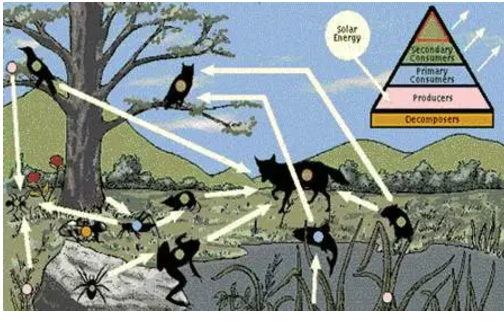
\includegraphics[scale=0.6]{pic/stnetwork.png}
}

\frame{\frametitle{传染病模型 意义}
	医学科学的发展已经能够有效地预防和控制许多传染病,但是仍然有一些传染病暴发或流行,危害人们的健康和生命。
	
	~
	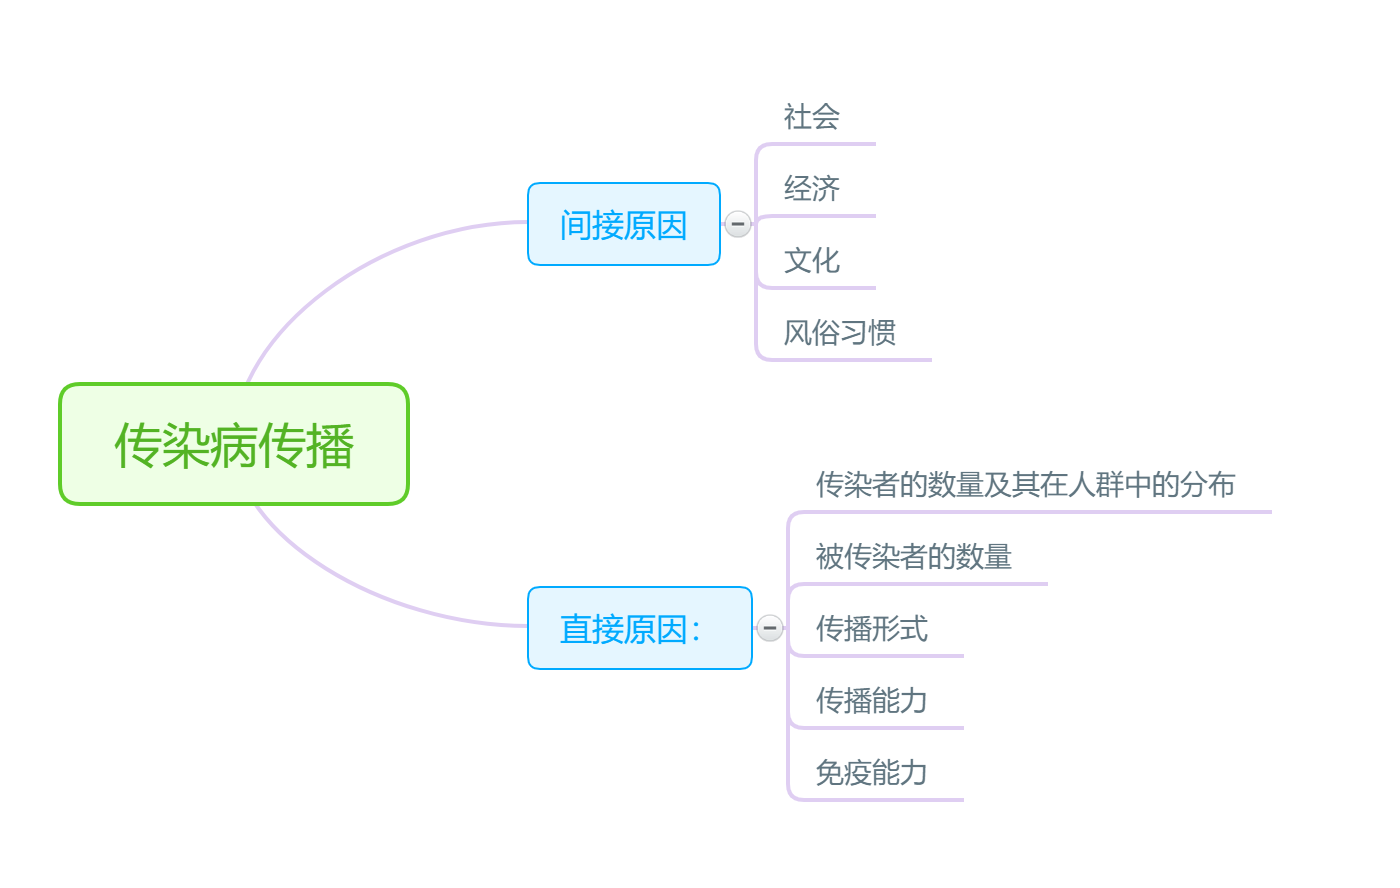
\includegraphics[scale=0.6]{pic/sp.png} 
	
}
\frame{\frametitle{模型分类}
	人群分成三类:
	\begin{itemize}
		\item<1-> S类,易感者(Susceptible),指未得病者,但缺乏免疫能力,与感染者接触后容易受到感染;
		\item<2-> I类,感病者(Infective),指染上传染病的人,它可以传播给S类成员;
		\item<3-> R类,移出者(Removal),指被隔离或因病愈而具有免疫力的人
	\end{itemize} 
	~
	SI模型
	~
	SIS模型
	~	
	SIR模型
	
	
}
\frame{\frametitle{模型假设和默认条件}
	模型假设
	~
	\begin{itemize}
		\item<1-> 1,Compartmentalization;
		\item<2-> 2, Homogenous Mixing
	\end{itemize} 
	~
	默认条件
	~
	\begin{itemize}
		\item<3-> 1, closed population; 
		\item<4-> 2, no births;
		\item<5-> 3, no deaths;
		\item<6-> 4, no migrations
	\end{itemize} 
}
\frame{\frametitle{SI}
	只有健康人才可以被传染为病人,不考虑治愈。
	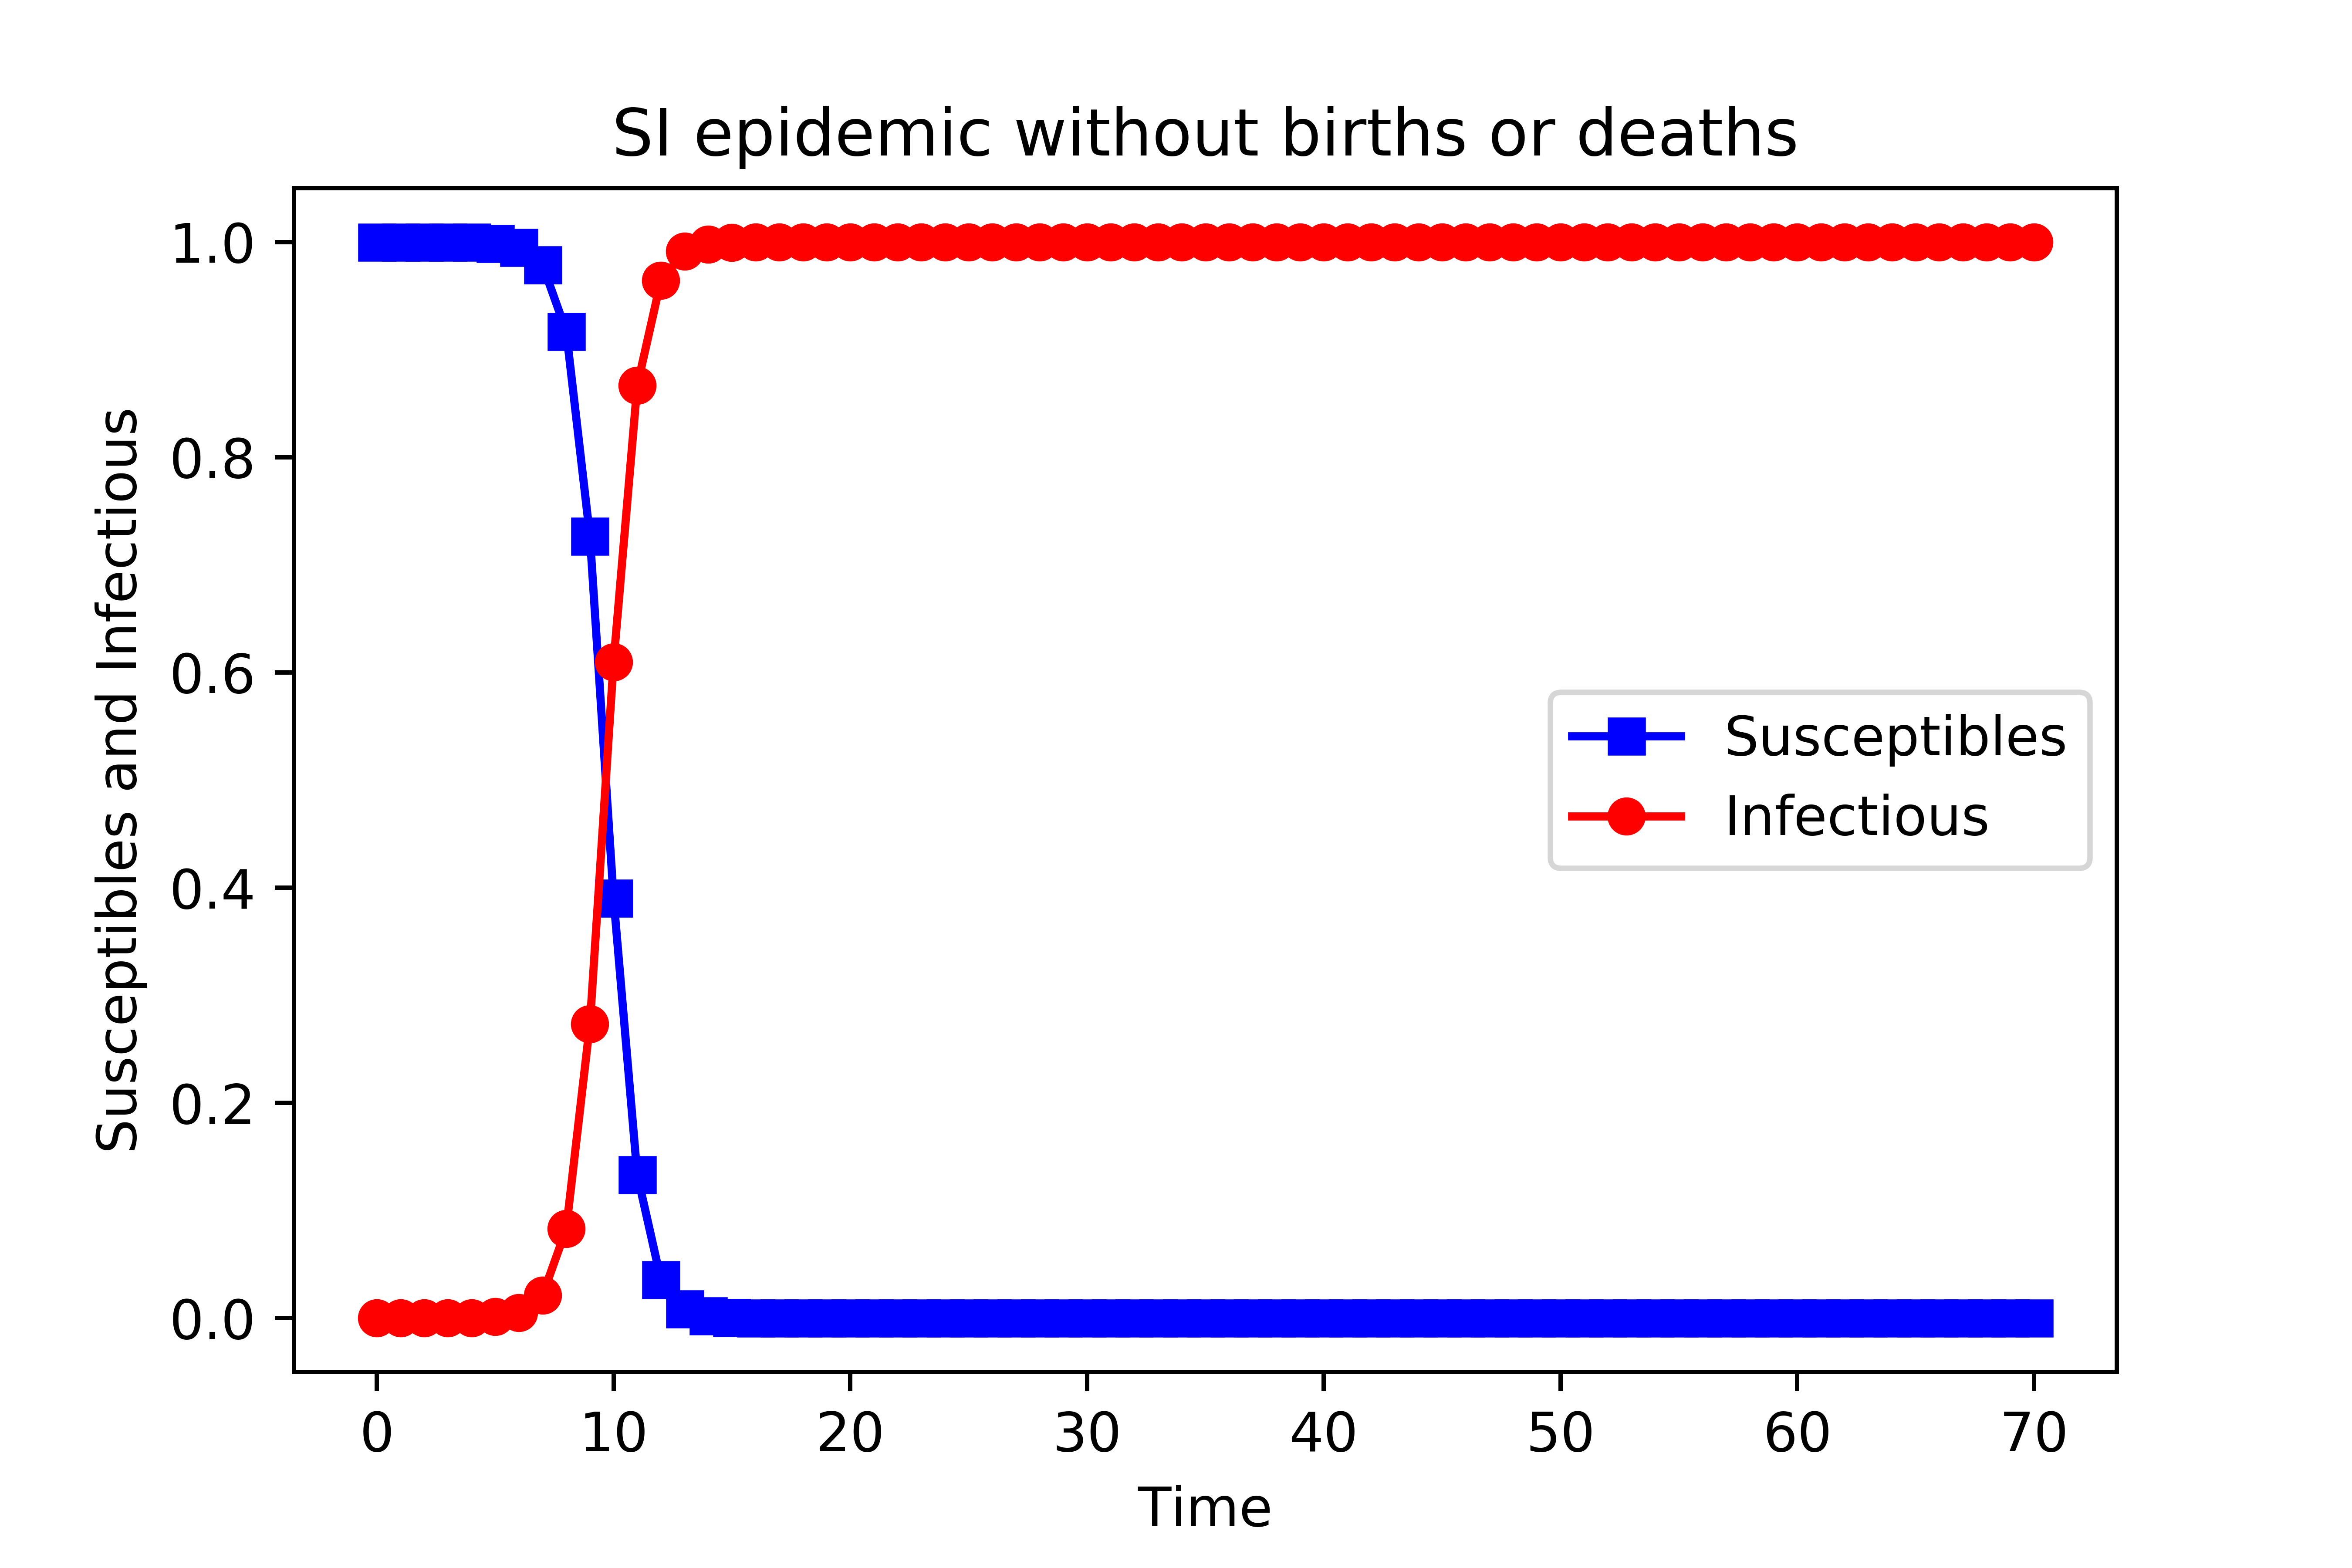
\includegraphics[scale=0.6]{pic/SI.png}
	
}

\frame{\frametitle{SIS}
	有些传染病如伤风、痢疾等愈合后免疫力很低,假定无免疫力。起初你容易感染某一种疾病并确实被感染,得到治疗并痊愈,但是你再一次面临被传染的风险。
	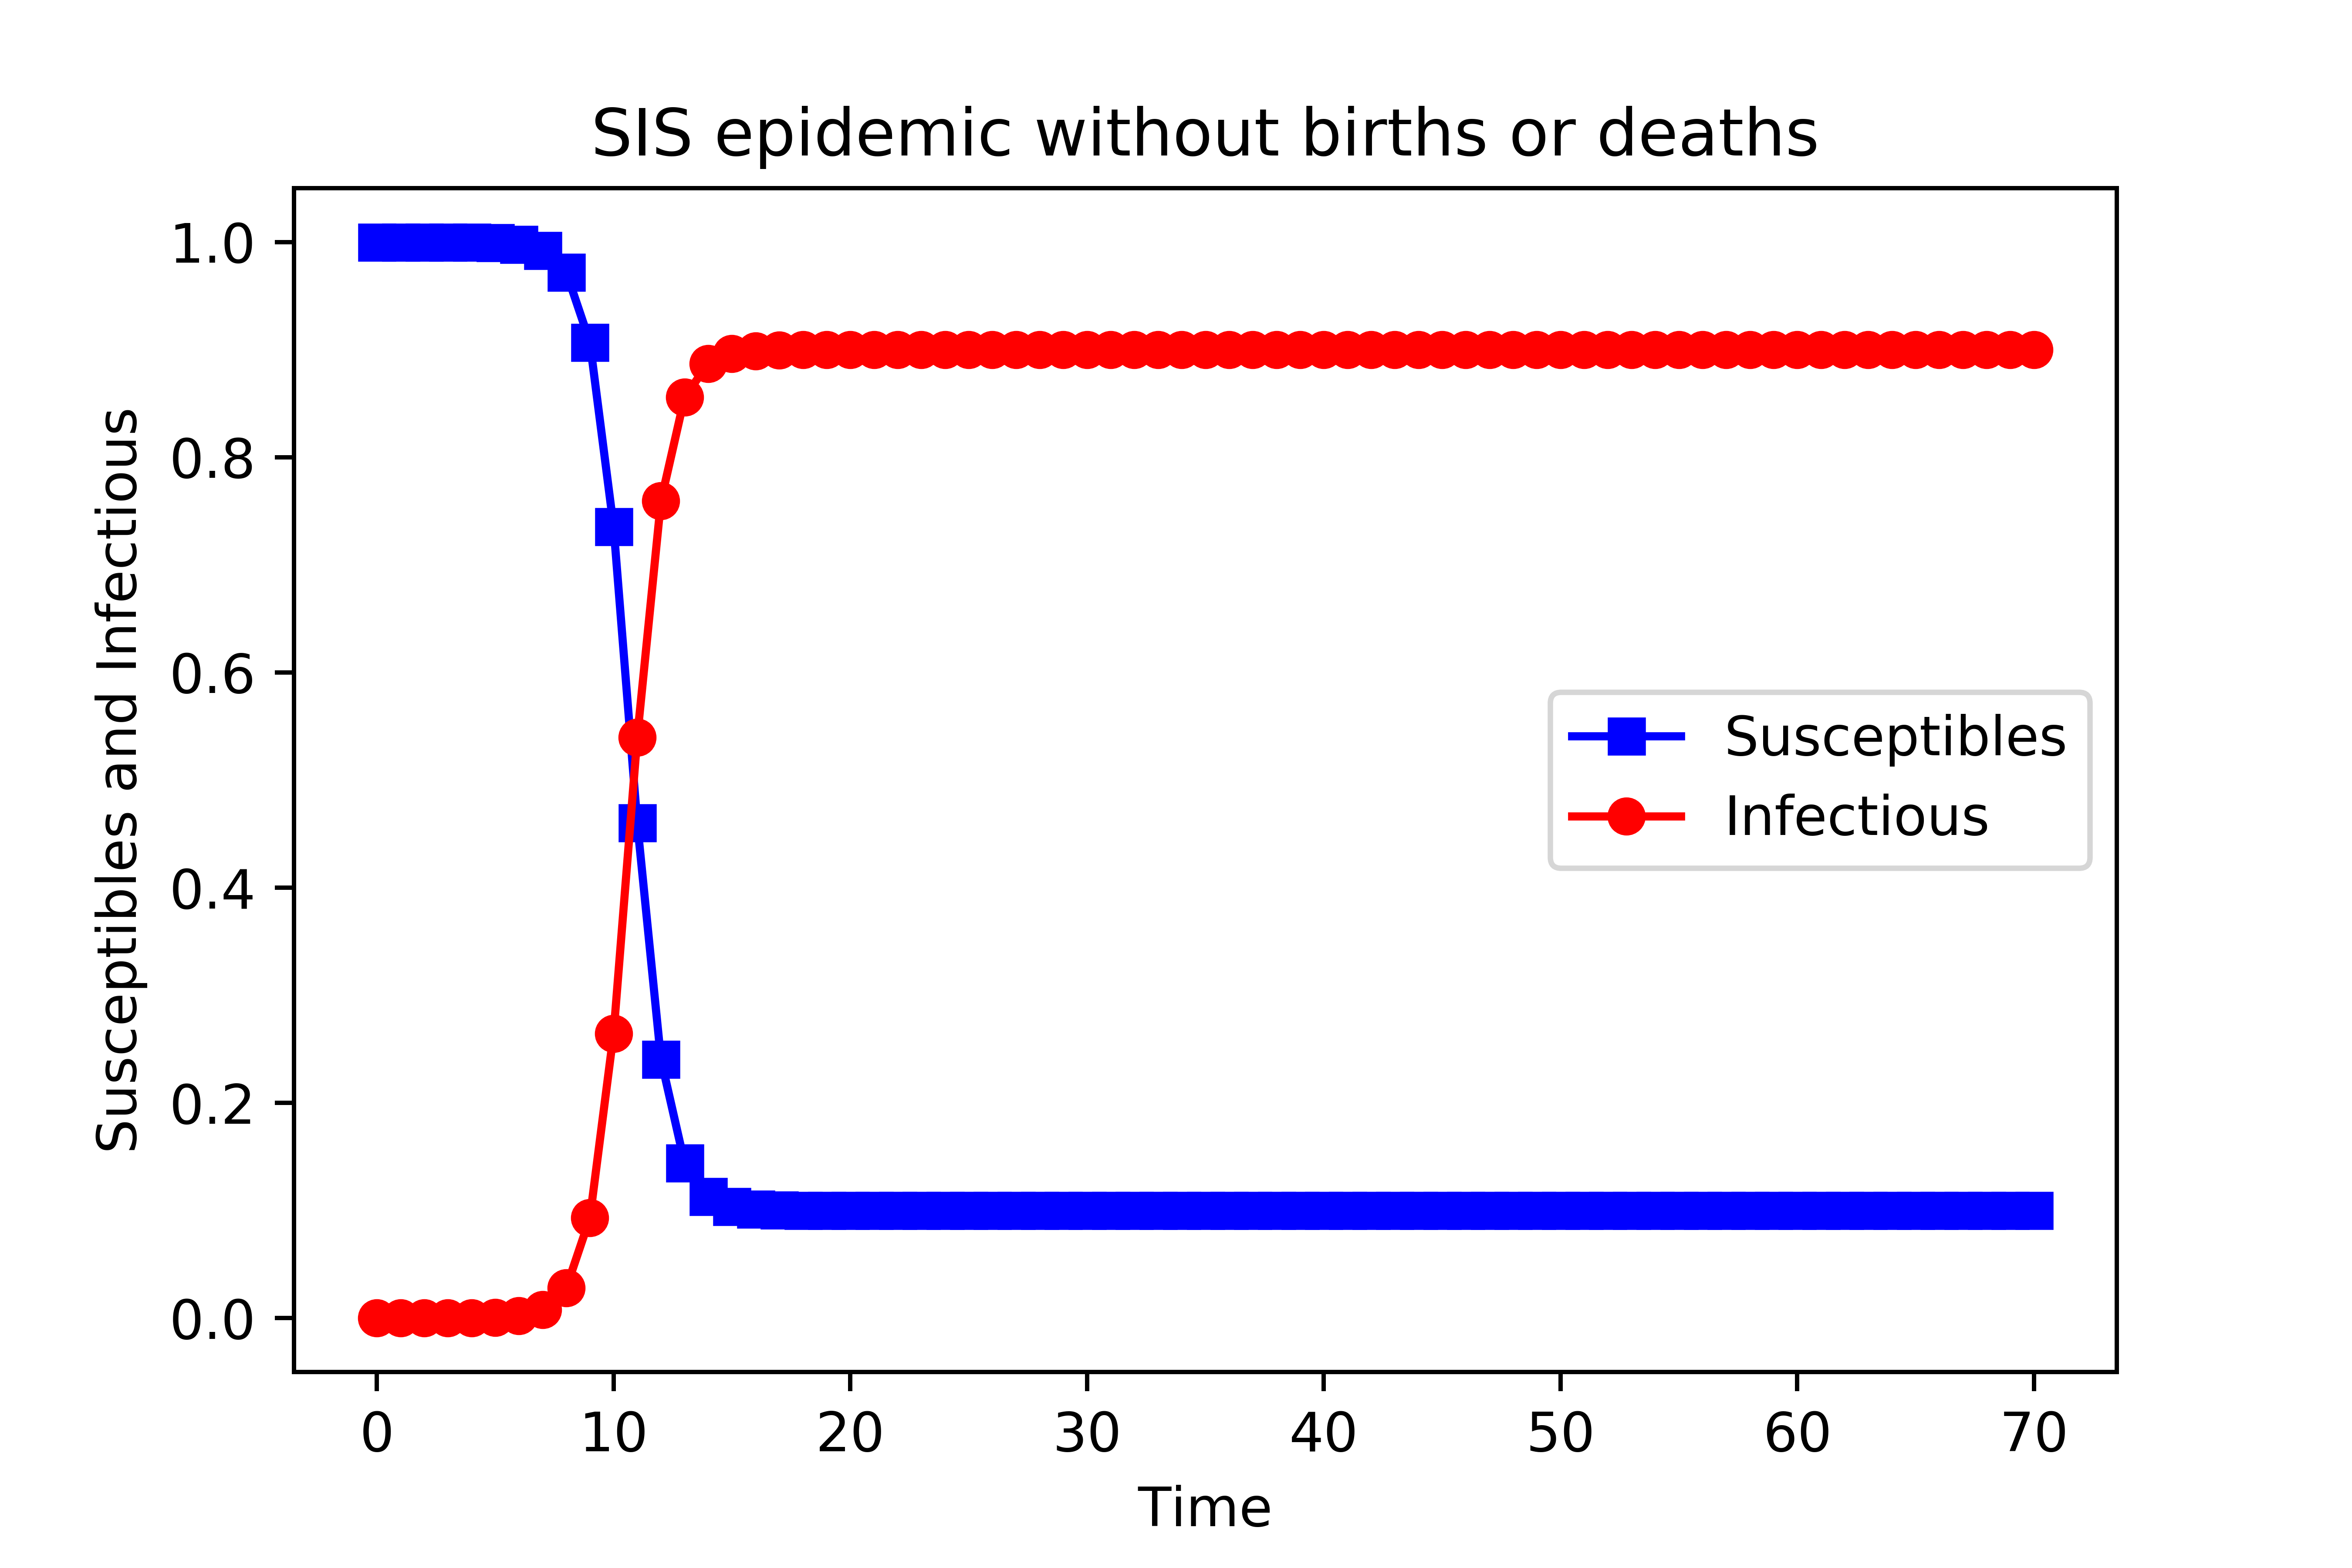
\includegraphics[scale=0.6]{pic/SIS.png} 
}

\frame{\frametitle{SIR}
	适用于那些使传染者感染后可以得到免疫力的例子。健康人被感染之后被治愈,然后会对这种疾病产生抗性并不会再被感染。
	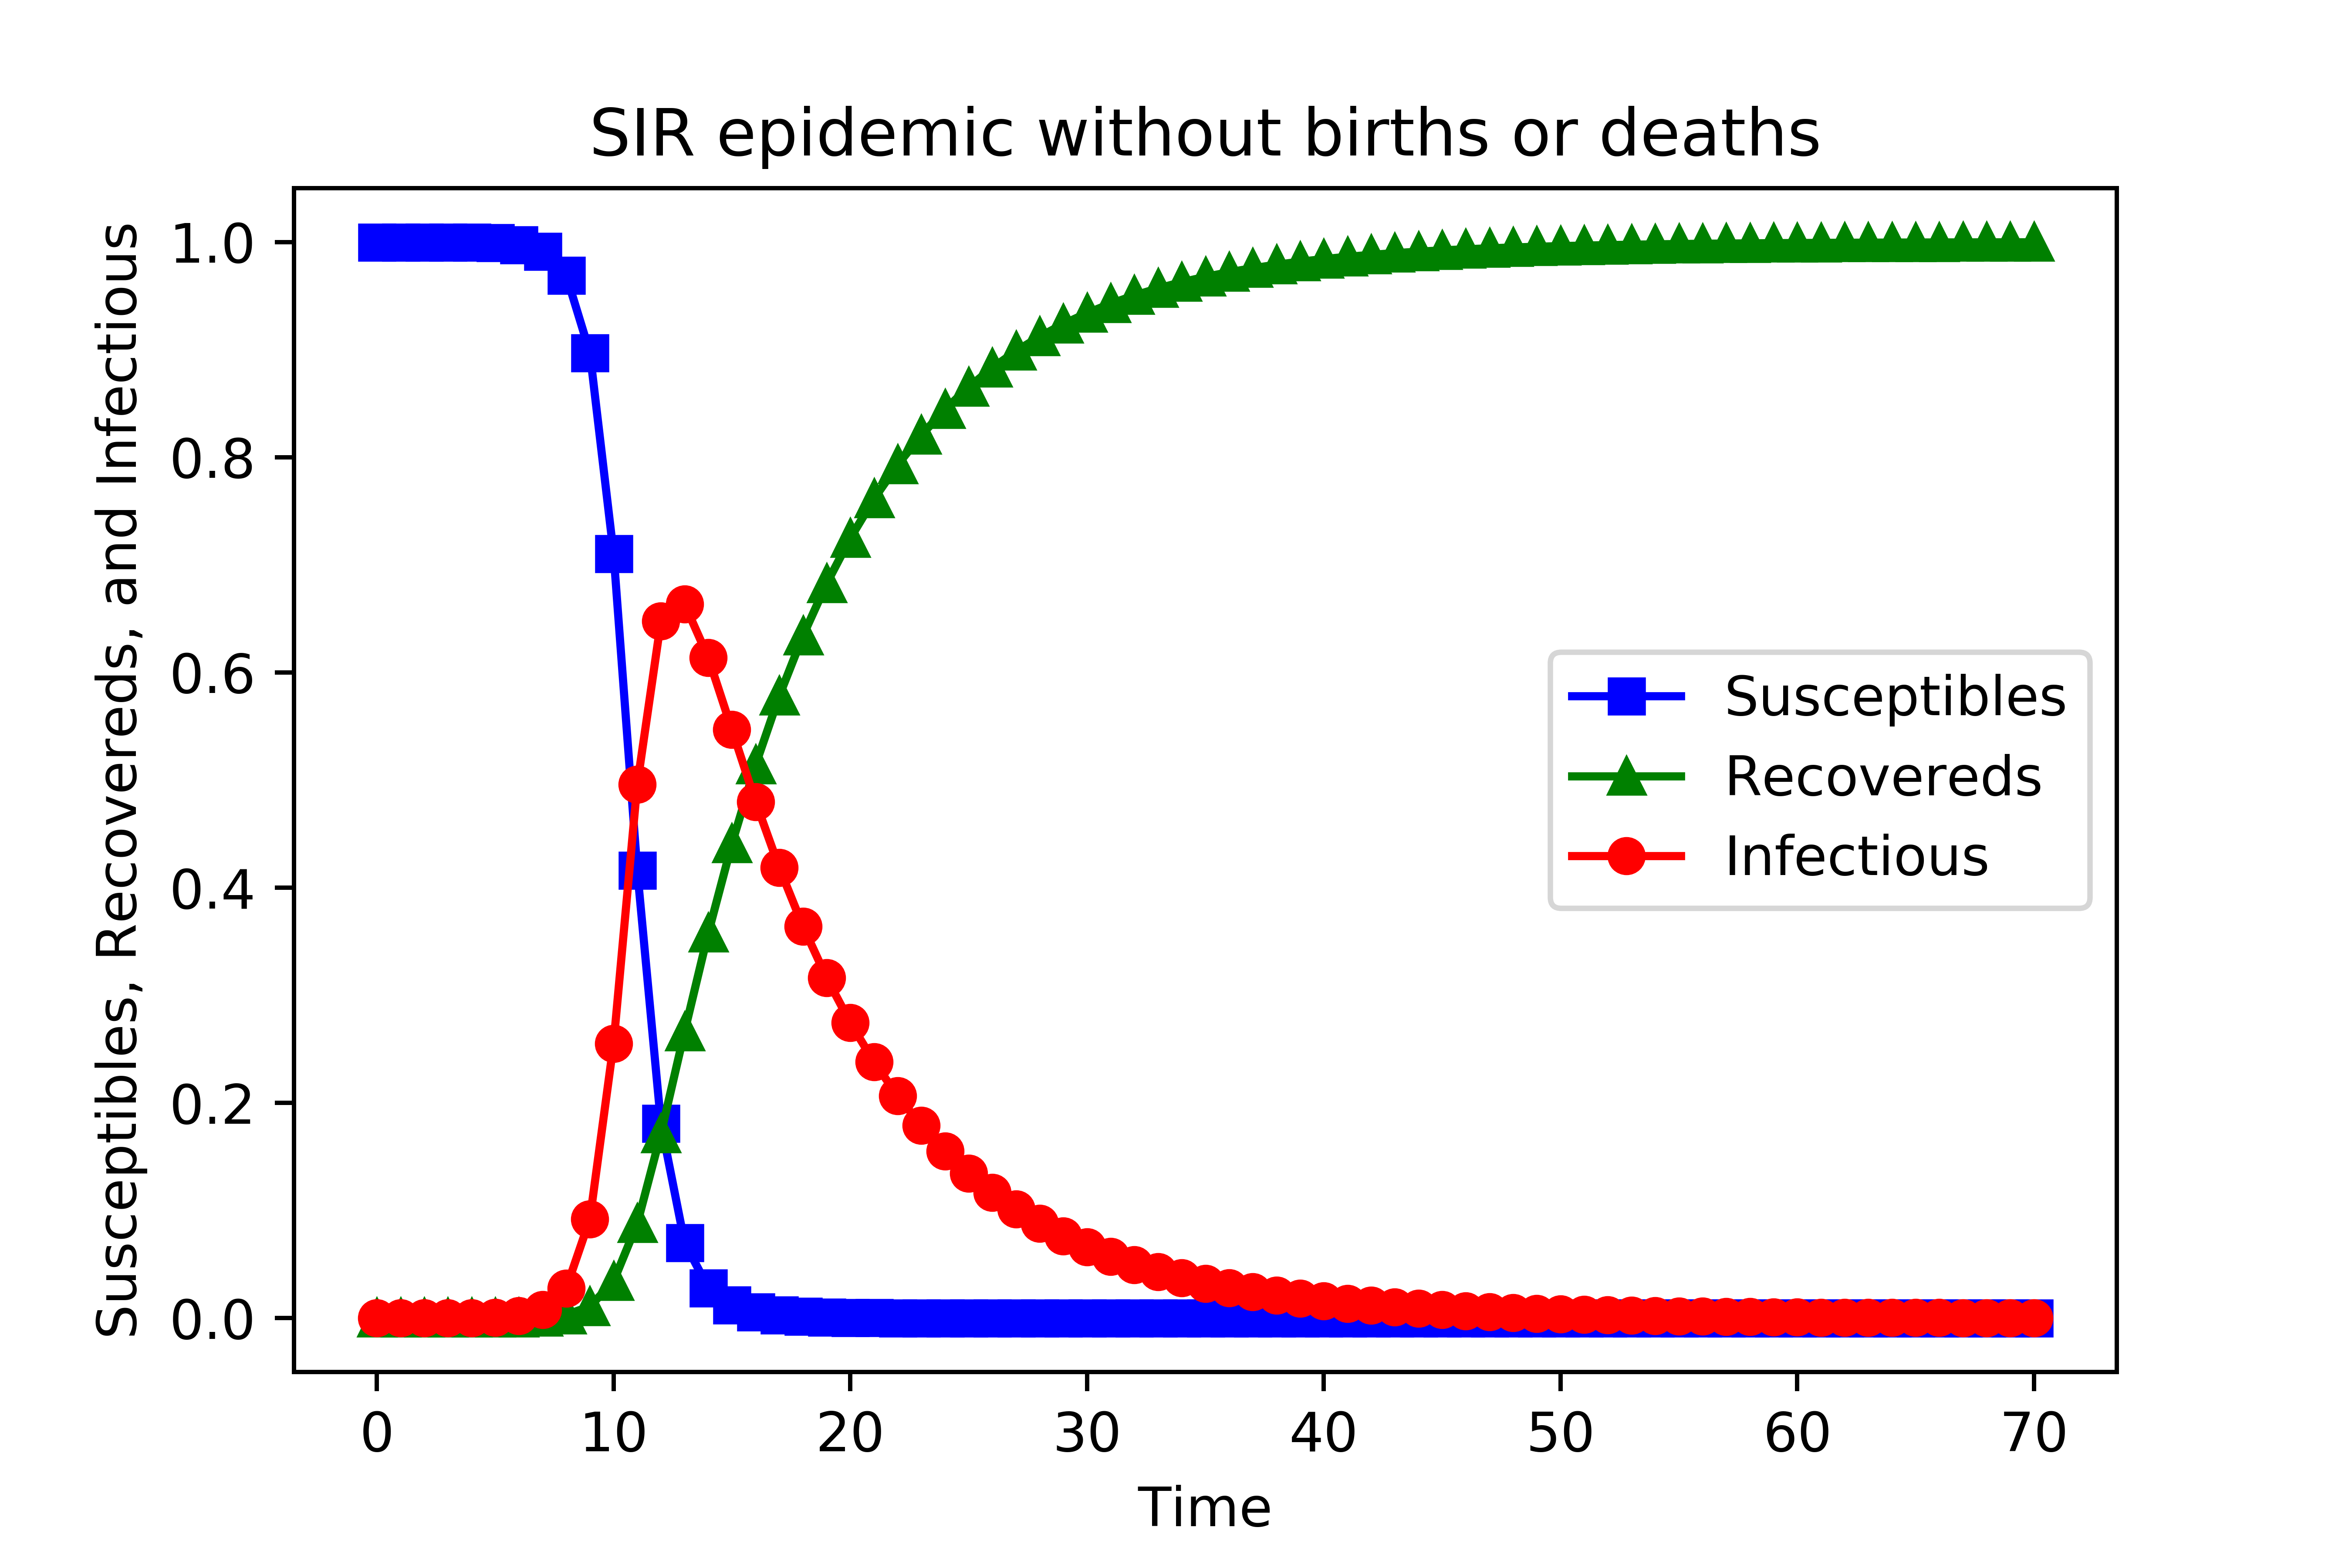
\includegraphics[scale=0.6]{pic/SIR.png} 
}


%end
